%%%%%%%%%%%%%%%%%%%%%%%%%%%%%%%%%%%%%%%%%%%%%%%%%%%%%%
\documentclass[12pt,a4paper,oneside]{report}

%%%%%%%%%%%%%%%%%%%%% packages %%%%%%%%%%%%%%%%%%%%%
\usepackage[french]{babel} 
\usepackage[utf8]{inputenc}
\usepackage[T1]{fontenc}

\usepackage[table]{xcolor} %for colors

\usepackage{graphicx} % images, colors, etc
\usepackage[toc]{glossaries} % glossaries
\usepackage{pdfpages} % include pdf file in document
\usepackage{hyperref} % for references
\usepackage{float} % align figure
\usepackage{adjustbox}

\usepackage{tikz}% for diagram
\usetikzlibrary{shapes.geometric, arrows}

\usepackage{multirow} % mutliple row in tabular
\usepackage{hhline} % double hline in tabular


%\usepackage{pstricks}
%\usepackage{auto-pst-pdf}

%\usepackage{enumitem}% control layout of the three basic list environments.



\usepackage{fancyhdr} % page style

%%%%%%%%%%%%%%%%%%%%% page style %%%%%%%%%%%%%%%%%%%%%
\pagestyle{fancy}

\setlength{\parindent}{1cm}
\newcommand{\textcalli}[1]{{\small{\textbf{$\negmedspace$\calligra #1}}}}

\renewcommand{\chaptermark}[1]{\markright{\thechapter\ #1}}
\renewcommand{\sectionmark}[1]{\markright{\thesection\ #1}}
\fancyhf{} % supprime les en-têtes et pieds prédéfinis
\fancyhead[R]{\thepage}% Left Even, Right Odd
%\fancyhead[R]{\textsl{\rightmark}}%moi
\fancyhead[L]{\textsl{\leftmark}} % Left Odd
%\fancyfoot[R]{\thepage} %moi
%\fancyhead[RE]{\textsl{\leftmark}} % Right Even
\renewcommand{\headrulewidth}{0pt}% filet en haut de page
\renewcommand{\footrulewidth}{0pt} % pas de filet en bas
\fancypagestyle{plain}{ % pages de tetes de chapitre
\fancyhead{} % supprime l’entete
\fancyhead[R]{\thepage}
\renewcommand{\headrulewidth}{0pt} % et le filet
}
%\makeglossaries
%\loadglsentries{glossaire.tex}

%%uses bullets for itemize
\AtBeginDocument{\def\labelitemi{$\bullet$}}

%%colors
\definecolor{dark}{HTML}{333333}
\definecolor{red}{HTML}{D1002E}
\definecolor{grey}{HTML}{888A8D}
\definecolor{white}{HTML}{FFFFFF}
\definecolor{blue}{HTML}{00ABD0}
\definecolor{green}{HTML}{00C048}

%%Flowcharts
%\tikzstyle{mydecision}=[diamond, draw=black, fill=grey, text=white!30, text centered, node distance=3cm]
\tikzstyle{endfail} = [rectangle, rounded corners, minimum width=3cm, minimum height=1cm,text centered, draw=black, fill=red]
\tikzstyle{endsuccess} = [rectangle, rounded corners, minimum width=3cm, minimum height=1cm,text centered, draw=black, fill=green]
\tikzstyle{process} = [rectangle, minimum width=3cm, minimum height=1cm, text centered, draw=black, fill=grey!30]
\tikzstyle{decision} = [diamond, minimum width=3cm, minimum height=1cm, text centered, draw=black, fill=dark!60]
\tikzstyle{arrow} = [thick,->,>=stealth]
 % load theme
%%%%%%%%%%%%%%%%%%%%%%%%%%%%%%%%%%%%%%%%%%%%%%%%%%%%%%
%%%%%%%%%%%%%%%%%%%%%%%%%%%%%%%%%%%%%%%%%%%%%%%%%%%%%%
\begin{document}

%%%%%%%%%%%%%%%%%%%%% title page %%%%%%%%%%%%%%%%%%%%%
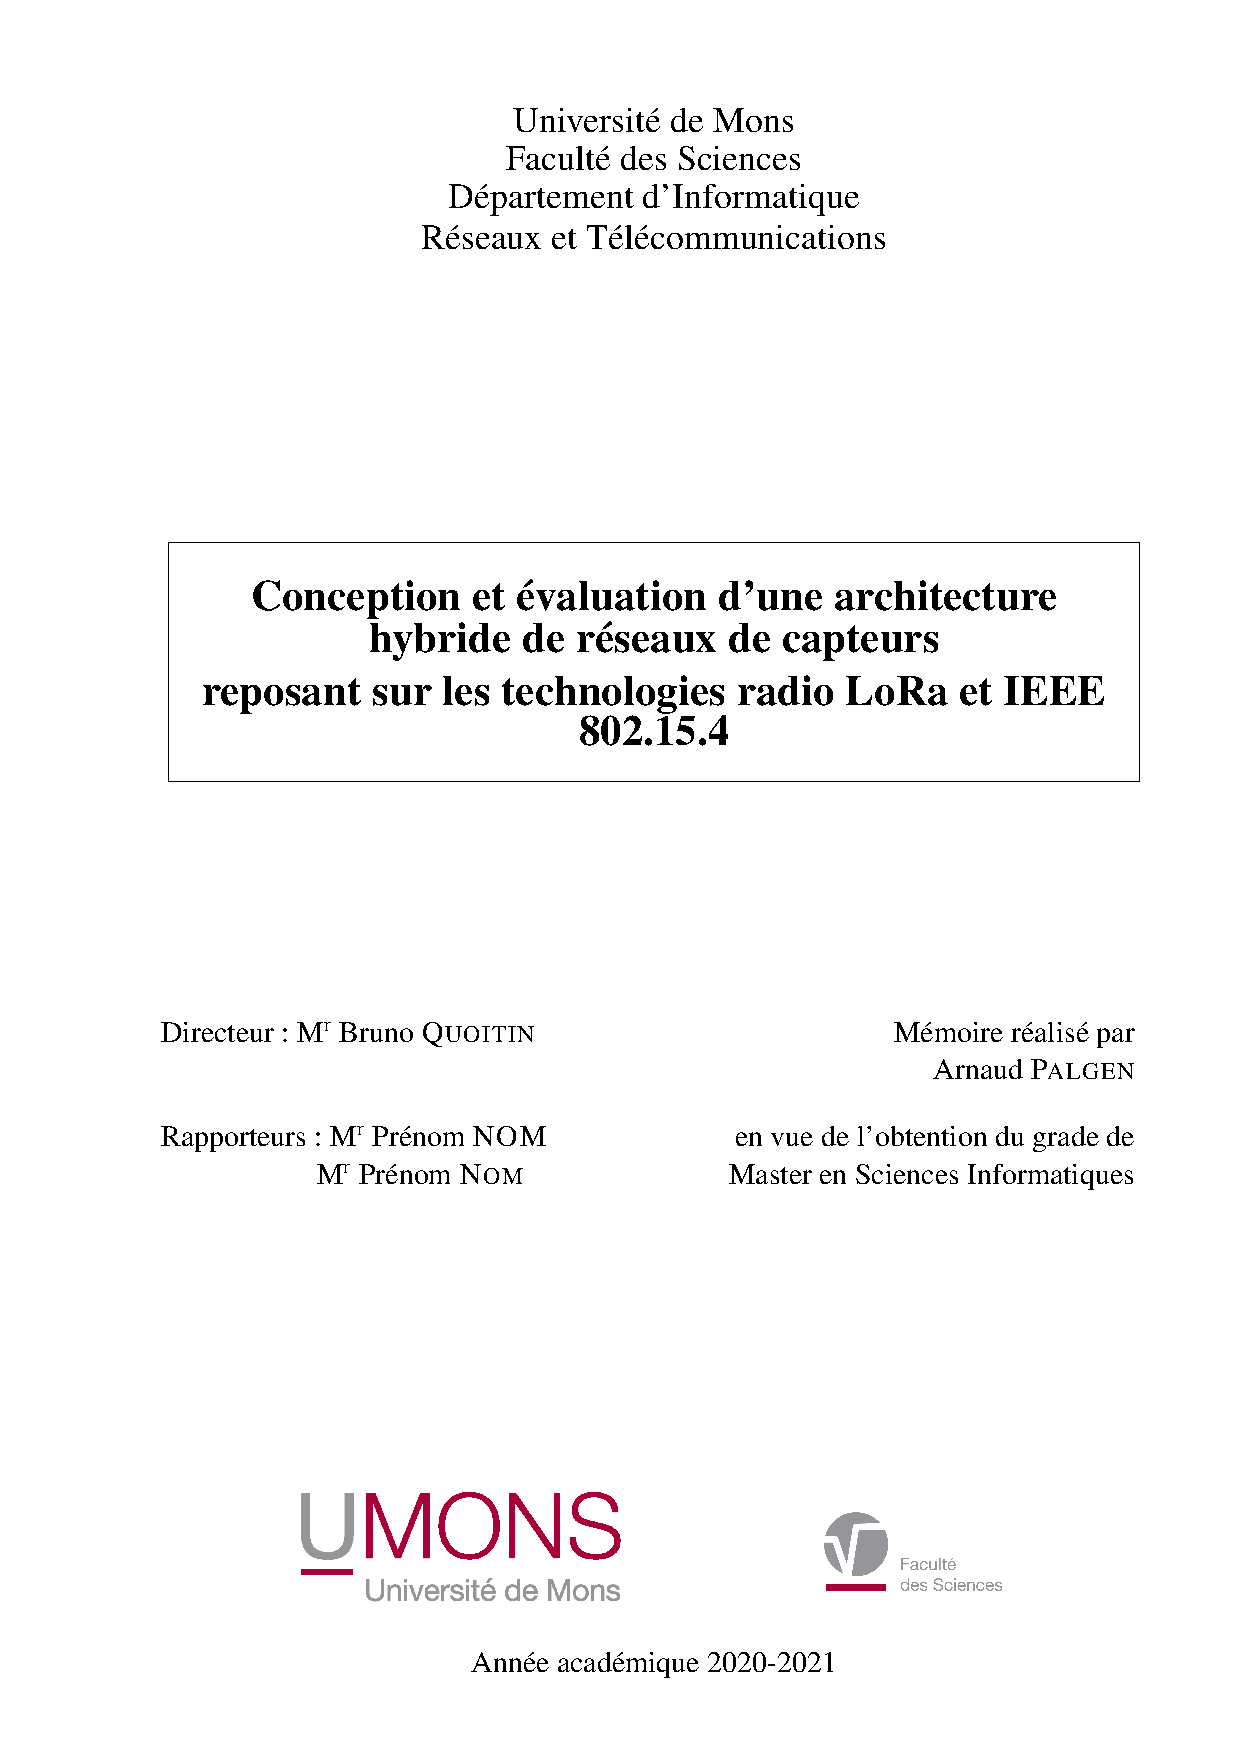
\includepdf[pages=-]{page_garde/page_garde.pdf}

\pagenumbering{roman}

%%%%%%%%%%%%%%%%%%%%% thanks %%%%%%%%%%%%%%%%%%%%%
\chapter*{Remerciements}
\renewcommand{\leftmark}{REMERCIEMENTS}

    Nous remercions ...\\

\newpage

%%%%%%%%%%%%%%%%%%%%% table of contents %%%%%%%%%%%%%%%%%%%%%
\renewcommand{\leftmark}{TABLE DES MATI\`{E}RES}
\thispagestyle{fancy}
\tableofcontents

\newpage
\listoffigures
\pagenumbering{arabic}
%%%%%%%%%%%%%%%%%%%%% intro %%%%%%%%%%%%%%%%%%%%%
%L’objectif de ce mémoire est la conception d’une architecture de réseaux de capteurs utilisant deux
technologies de transmission radio différentes : LoRa et IEEE 802.15.4.

Le déploiment de cette architecture est envisagée pour la surveillance de cultures dont la topographie
est difficile.

Les contraintes de ce projet sont les suivantes:
\begin{itemize}
    \item Les noeuds du réseau sont fortement contraints énergétiquement. Ils seront typiquement alimentés
    par une batterie éventuellement associée à des panneaux solaires et un régulateur de charge.
    \item Les caractéristiques des liens radio LoRa et IEEE 802.15.4 sont différentes et susceptibles
    de changer au cours du temps suite à par exemple, la croissance des feuilles des cultures surveillées.
\end{itemize}
\newpage
%%%%%%%%%%%%%%%%%%%%% content %%%%%%%%%%%%%%%%%%%%%
\section{Plateformes de développement}\label{sec:etat_art-802.15.4}
\renewcommand{\rightmark}{Plateformes de développement}
\subsection*{Zolertia RE-Mote}
Pour ce mémoire, la plateforme Zolertia RE-Mote revision B(Fig.~\ref{fig:state-zolertia}) est utilisée.

Cette plateforme, basée sur un system on chip (SoC) CC2538 ARM Cortex-M3, a été conçue par des universités et des industriels dans le but de permettre aux chercheurs et makers de développer des applications IoT et des objets connectés.

Le Zolertia RE-Mote a été choisi car elle est équipée de deux radios compatibles IEEE 802.15.4,
permet une consommation électrique faible et possède de nombreux pins de connexion qui peuvent être utilisés pour y connecter des capteurs, actuateurs, radios, etc.

Le prix du consturcteur pour cette plateforme est de 93,95€~\cite{zolertia-remote:shop}.

\begin{figure}[H]
    \centering
    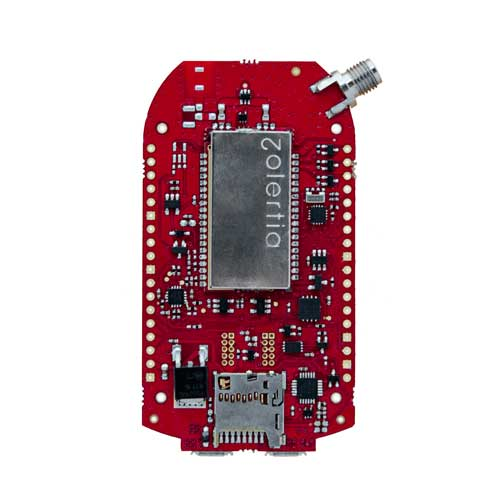
\includegraphics[scale=0.3]{res/pictures/remote-zolertia.jpg}
    \caption{Zolertia RE-Mote révision B~\cite{zolertia-remote:shop}.}
    \label{fig:state-zolertia}
\end{figure}

La table~\ref{tb:state-spec} reprend les principales spécifications du Zolertia RE-Mote rev.b et sa table ... la consommation électique.%TODO datasheet ???

\begin{table}[H]
    \centering
    \begin{tabular}{|c|c|}
        \hline
        \rowcolor{lightgray}
        Element            & Spécification\\
        \hline
        Radio              & Deux radios IEEE 802.15.4 à 2.4 GHz et 863-950 MHz\\
        \hline
        CPU                & ARM\textsuperscript{\tiny\textregistered} Cortex\textsuperscript{\tiny\textregistered} -M3 jusqu'à 32 MHz\\
        \hline
        RAM                & 32 KB (16 KB pour tous les Power Modes)\\
        \hline
        Flash programmable & 512KB\\
        \hline
        I/O                & RGB led, boutton user et reset, USB 2.0 à 12Mbps, Real-Time Clock\\
        \hline
    \end{tabular}
    \caption{Spécifications du Zolertia RE-Mote rev.b~\cite{zolertia-remote:datasheet}.}
    \label{tb:state-spec} reprend la consommation de courant du RN2483 
\end{table}

\subsection*{RN2483}
    Le RN2483 (Fig.~\ref{fig:state-rn2483}) est un modem LoRa compatible LoRaWAN$^{TM}$ basse énergie.
    La communication avec ce modem ce fait par des commandes ASCII envoyée via une interface UART. Il prend en charge les modulations FSK, GFSK et LoRa. Il possède également 14 GPIOs ??pour le contrôle et le status, partagés avec 14 inputs analogiques.??%TODO
    Ses fréquences opérationnelles sont situées dans les bandes de fréquences 433 MHz et 868 MHz. D'après la datasheet, 
    sa portée maximale est de 15km en agglomération et 5km en zone urbaine. Comme l'illustre la figure.~\ref{fig:state-rn2483}, pour ce mémoire, le RN2483 a été monté sur un carte d'interface réalisée par B.Quoitin qui comporte deux leds, une petite antenne ainsi que les connecteurs permettant d'utiliser des câbles de prototypages.

    \begin{figure}[H]%TODO changer figure
        \centering
        
\includegraphics[scale=0.3]{res/pictures/rn2483.png}
        \caption{RN2483~\cite{rn2483:shop}.}
        \label{fig:state-rn2483}
    \end{figure}

    La figure \ref{fig:state-rn2484-block} reprend le schéma-bloc du RN2483. Il contient notemment l'interface UART, les antennes 433 MHz et 868Mhz ainsi que les GPIOs et la stack LoRaWan.
    \begin{figure}[H]
        \centering
        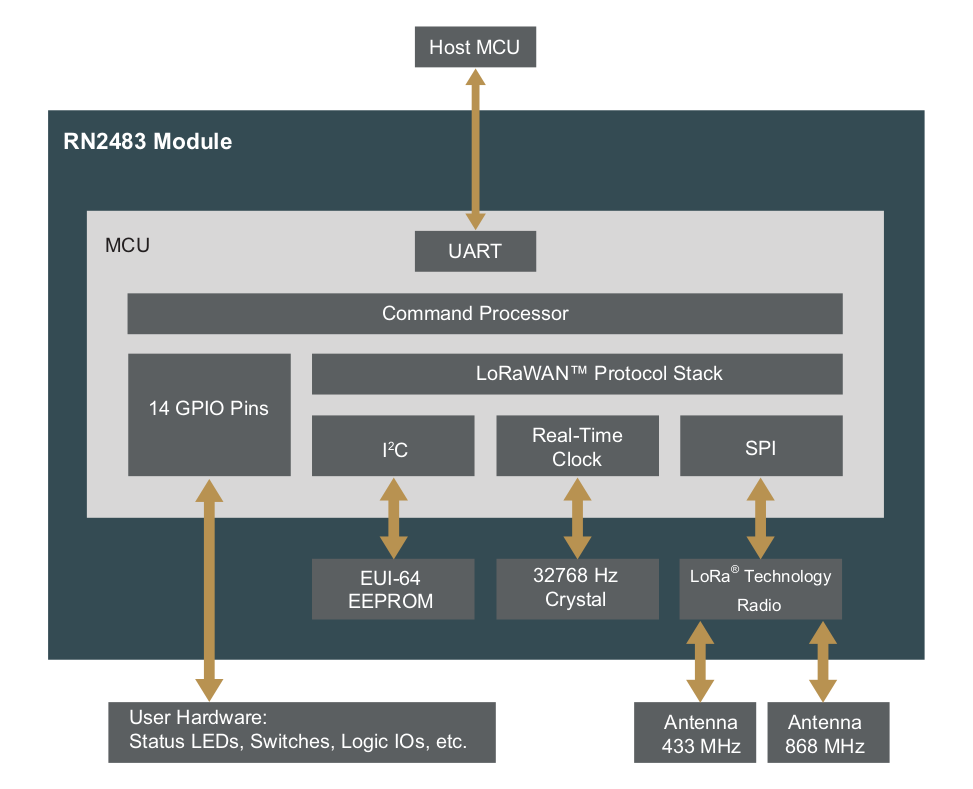
\includegraphics[scale=0.4]{res/pictures/rn2483-block-diagram.png}
        \caption{Schéma-bloc du RN2483~\cite{rn2483:datasheet}.}
        \label{fig:state-rn2484-block}
    \end{figure}
    La table~\ref{tb:state-rn2483-consumption} reprend la consommation électrique du RN2483 en fonction de son mode de fonctionnement.
    \begin{table}[H]
        \centering
        \begin{tabular}{| *{4}{c|} }
            \hline
            Mode & \multicolumn{3}{c|}{\multirow{1}{*}{Courant (mA)}}\\ \cline{2-4}
             & VDD = 2.1V & VDD = 3.3V  & VDD = 3.6V \\ \hhline{|=|=|=|=|}
            Idle & 1.7 & 2.8 & 3.1 \\ \hline
            Transmit & 28.6 & 38.9 & 44.5 \\ \hline
            Sleep & 0.0015 & 0.0016 & 0.0016 \\ \hline
            Receive & 12.96 & 14.22 & 14.69 \\ \hline
        \end{tabular}
        \caption{Consommation de courant (à 25 °C) \cite{rn2483:datasheet}.}
        \label{tb:state-rn2483-consumption}
    \end{table}

\subsection*{Raspberry Pi}

Le Raspberri Pi est un ordinateur monocarte. Le modèle utilisé pour ce projet est un Raspberry Pi 3 modèle B+ (Fig.~\ref{fig:state-raspberrypi}). La table \ref{tb:state-raspberrypi-spec} reprend les principales caractéristiques de ce modèle.

\begin{figure}[H]
    \centering
    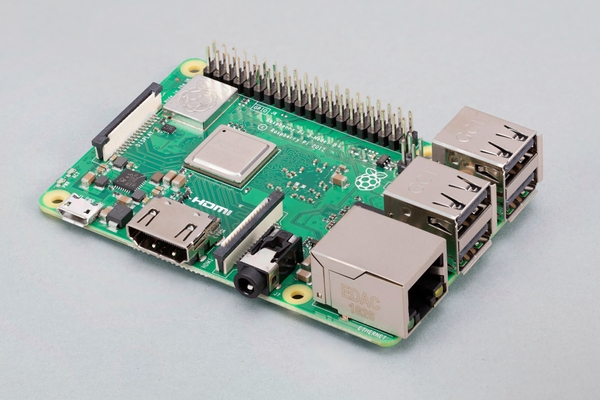
\includegraphics[scale=0.4]{res/pictures/raspberrypi3b+.png}
    \caption{Raspberry Pi 3B+~\cite{raspberry:shop}.}
    \label{fig:state-raspberrypi}
\end{figure}

\begin{table}[H]
    \centering
    \begin{tabular}{|c|p{0.75\textwidth}|}
        \hline
        \rowcolor{lightgray}
        Element            & Spécification\\
        CPU & Broadcom BCM2837B0, Cortex-A53 64-bit SoC à 1.4GHz\\ \hline
        Mémoire & 1GB LPDDR2 SDRAM \\ \hline
        Connectivité & 
        \begin{itemize}
            \item IEEE 802.11.b/g/n/ac, Bluetooth 4.2, BLE
            \item Gigabit Ethernet over USB 2.0
            \item 4 × USB 2.0 ports
        \end{itemize}\\ \hline
        Alimentation & 5V/2.5A DC\\ \hline
    \end{tabular}
    \caption{Spécifications du Raspberry Pi 3B+ \cite{raspberry:shop}.}
    \label{tb:state-raspberrypi-spec}
\end{table}

\newpage
\section{RTOS}

Un RTOS (Real Time Operating System) est un sytème d'exploitation temps réels principalement destiné aux systèmes embarqués.

Etant donné que ce projet utilise le protocole 802.15.4 ainsi que TSCH, le RTOS choisis doit les prendre en charge ainsi qu'un ou plusieurs algorithme d'ordonnancement de TSCH

Il est également préférable, que le RTOS choisis, supporte déjà la plateforme utilisée. Une implémentation de la LoRa n'est pas nécessaire car les communications Lora sont réalisées via le RN2483 qui est controlé par UART.

Pour effectuer ce choix, les RTOS suivants ont été comparés: Contiki OS, FreeRTOS, RIOT OS et Zephyr.

\subsection*{Contiki OS}
    Le développement publique de Contiki a débuté en octobre 2012\footnote{Date de création du repository Github.} Dans un premier repository: contiki~\cite{contiki-repo:old}. Un nouveau développement a démarré en mai 2017 sous le nom de Contiki-NG~\cite{contiki-repo:ng}. C'est donc ce dernier qui est utilisé pour la comparaison est qui est dénommé par la suite Contiki.

    Cet OS open-source et multi-plateforme implémente toute une série de protocoles de communications basse énergie tels que IEEE 802.15.4, 6TiSCH, IPv6/6LoWPAN et RPL. En plus de 6TiSCH, un ordonnanceur TSCH, Orchestra, est implémenté.
    TODO udp/tcp

    Contiki est également compatible avec le Zolertia RE-Mote. Il est accompagné de Cooja, un simulateur réseau qui permet de simuler les communications entre plusieurs noeuds utilisant Contiki.

\subsection*{FreeRTOS}
    D'après le site officiel de FreeRTOS~\cite{freertos}, ce RTOS est développé depuis 15 ans.
    TODO compatible avec zolertia ?

    \subsection*{RIOT OS}
    Le développement publique de RIOT a débuté en décembre 2012\footnotemark[1].
    
    D'après le site officiel, cet OS supporte 229 carte de développement et 64 CPU dont le Zolertia RE-Mote. 

    La pile réseau de RIOT comporte les protocoles notemment 6LoWPAN, IPv6, RPL, LoRaWan, 802.15.4.

\subsection*{Zephyr}
    TODO

Le table~\ref{tb:state-rtos-choice} résume la comparaison de ces RTOS.

Le RTOS choisi est Contiki OS. Il a été choisi pour sa maturié, la prise en charge du Zolertia RE-Mote et sa pile réseau complète.


%https://github.com/Lora-net/LoRaMac-node/blob/ba17382bd5109513937afad07f068a781a503ef6/src/radio/radio.h
\begin{table}[H]
    \begin{adjustbox}{width=\textwidth}
        \begin{tabular}{c||c|c|c|c|c|c|c}
            RTOS & 802.15.4 & ord. TSCH & LoRa & IPv6 & routage IP & comp. \\ \hline

            \textbf{Contiki OS} & $\surd$  & 6Tisch, Orchestra & Projet KRATOS & $\surd$ & RPL        & $\surd$ \\ \hline

            FreeRTOS            & $\times$ & $\times$          & $\surd$       & $\surd$ & $\times$   &    $\times$     \\ \hline

            RIOT OS             & $\surd$  & $\times$          & $\surd$       & $\surd$ & RPL        &    $\surd$     \\ \hline

            Zephyr              & $\surd$  & $\times$          & $\surd$       & $\surd$ & Thread     &    $\times$     \\
        \end{tabular}
    \end{adjustbox}
    \caption{Comparatif de différents RTOS.}
    \label{tb:state-rtos-choice}
\end{table}
%\section{IEEE 802.15.4e}\label{sec:etat_art-802.15.4}
\renewcommand{\rightmark}{IEEE 802.15.4e}
    802.15.4 est un protocole définis par IEEE en 2003. Il est destiné aux communications à débit faibles réalsisées par des dispositifs ayant une alimentation en énergie limitée.
    Ce protocole qui est un standart pour les réseaux PANs (Personak Area Networks) couvre la couche physique et MAC du modèle OSI. En 2012, IEEE 802.15.4e a été défini pour palier à certains problèmes de IEEE 802.15.4.

\subsection*{IEEE 802.15.4}
    \subsubsection*{Types de noeuds et topologie}
    Cette norme défini deux types de noeuds: les Full Function Devices (FFD) qui peuvent être des coordinateurs de PAN, de simple coordinateurs ou de simple noeuds et les Reduced Function Device (RFD) qui utilisent une implémentation réduite du protocole et ne peuvent être que de simples noeuds.

    Ces noeuds peuvent former des réseaux suivantes plusieurs topologies
    comme la topologie en étoile pour laquelle plusieurs RFD sont connectés à un FFD qui
    joue le rôle de coordinateur ou encore la topologie peer-to-peer pour laquelle les FFD sont connectés les uns aux autres.

    \subsubsection*{Modes d'accès}
    802.15.4 défini deux modes d'accès: Beacon Enabled mode et Non-Beacon Enabled mode.
    Dans le premier, le réseau est synchronisé par des messages de contrôles (beacons)
    et une structure appelée Superframe.

    Comme l'illustre la figure~\ref{fig:etat_art-802.15.4.superframe}, Cette Superframe est divisée en deux périodes: la période active et la période inactive. La période active est elle-même divisée en deux périodes: contention acces period (CAP) et contention free period (CFP). Dans la première, l'accès au canal se fait par l'algorithme CSMA-CA (Carrier Sense Multiple Access with Collision Avoidance).
    
    Dans la deuxième, l'accès au canal se fait par TDMA (Time Division Multiple Access). C'est à dire que les 7 slots de cette période sont attribués par le coordinateur aux noeuds ayant émis une requête durant la CAP pour l'utilisation d'un slot.

    \begin{figure}[H]
        \centering
        \makebox[\textwidth]
        {
          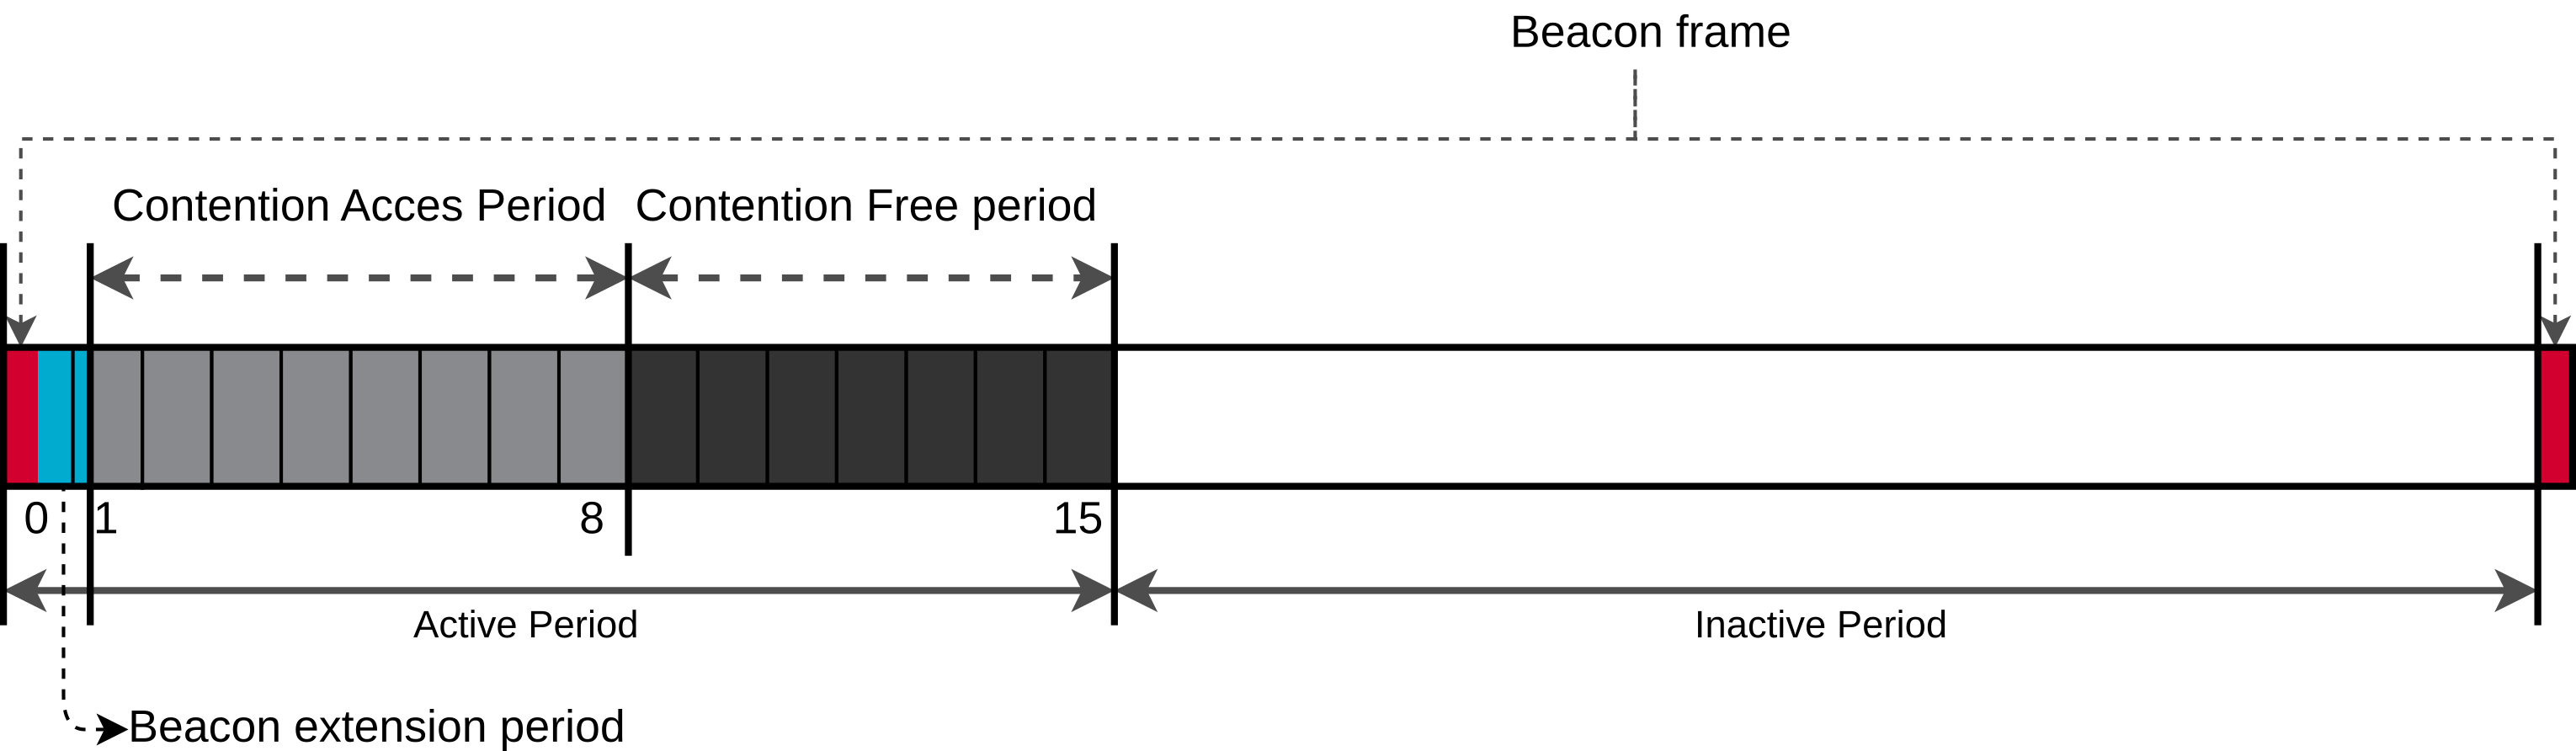
\includegraphics[scale=0.8]{res/pictures/superframe.png}
        }
        \caption{802.15.4 structure de la Superframe.}
        \label{fig:etat_art-802.15.4.superframe}
    \end{figure}

    Dans le mode Non-Beacon Enabled, il n'y a pas de synchronisation. l'accès au canal se fait par l'algorithme Unslotted CSMA-CA.


\subsection*{IEEE 802.15.4e}
    802.15.4 a un certains nombres de limitations. \cite{paper:802.15.4e-survey} met les limitations suivantes en évidence:
    \begin{itemize}
      \item Aucune garantie sur le délai maximal pour qu'un paquet puisse atteindre sa destination
        ne peut être fourni avec l'alorithme CSMA-CA.
      \item La fiabilité des communications est limitée par l'utilisation de l'algorithme slotted   CSMA-CA qui offre un taux de transmission faible.
      \item Aucune protection contre les interférences due à l'utilisation d'un seul canal et à     l'absence de mécanismes de sauts de fréquence (frequency hopping)
    \end{itemize}
    Ces limitations ont menées à la création de 802.14.4.e en 2012 qui redifinis les protocoles MAC du  standard.
    Ainsi, 5 modes de fonctionnement de la couche MAC sont introduis:
    \begin{enumerate}
      \item Time Slotted Channel Hopping (TSCH)
        %Cible les applications tel que l'automatisation de processus. Permet des communications    %multi-sauts et multi-canaux.
      \item Deterministic and Synchronous Multi-channel Extension (DSME)
        %Réalisé pour des applications industirelles et commercialesayant des contraintes de délai et
        %fiabilité. Permet des communications multi-sauts ainsi que la création de réseaux MESH.
      \item Low Latency Deterministic Network (LLDN)
        %Conçu pour les applications nécessitant une latence faible et les réseaux n'utilisant qu'un seul
        %canl pour des chemins d'un saut maximum.
      \item Asynchronous multi-channel adaptation (AMCA)
        %Cible les applications où de grands déploiments sont nécessaire comme le monitoring    %d'infrastructures.
      \item Radio Frequency Identification Blink (BLINK)
        %Conçu pour i'identification de personnes ou d'objets. Il permet aux noeuds de communiquer leur
        %ID aux autres noeuds sans avoir été préalablement associés.
    \end{enumerate}
    D'après \cite{paper:802.15.4e-survey}, le standart ne définit que brièvement AMCA et BLINK.
    LLDN est destiné aux réseaux à un seul saut et utilisant un seul canal. Il n'est donc pas pertinent pour ce projet. DSME utilise le concept de multi-superframe semblable aux superframe de IEEE 802.15.4 mise à part la CFP qui divie chacun des 7 slots en plusieurs fréquences.


\subsection{TSCH (Time Slotted Channel Hopping)}\label{subsec:etat_art-802.15.4.tsch}

Ce mode de fonctionnement de la couche MAC, comme son nom l'indique, supporte à la fois les sauts en fréquence et des communications divisées en temps. Ces mécanismes réduisent efficacement les effets des interférences et les collisions ce qui améliore la fiabilité du réseau.

\subsubsection*{Slotframe}
Dans ce mode, le concept de superframe de 802.15.4 est remplacé par le concept de slotframe.
Une slotframe est un intervalle de temps qui divisé en timeslots. Chaque timeslot permet à un noeud d'envoyer une trame et d'éventuellement recevoir son acquitement (ack).
Chaque timeslot possède un identifiant appellé \textit{Absolute Slot Number} (ASN)
et un identifiant au sein de la slotframe appelé \textit{Time Slot Number} (TSN).

TSCH permet l'utilisation de timeslots partagés et dédiés. Dans les timeslots partagés plusieurs noeuds peuvent communiquer. Dans ce cas, CSMA/CA est utilisé. Pour les timeslots dédiés, seul deux noeuds peuvent communiquer. La figure~\ref{fig:state-slotframe} illustre une slotframe composée de trois timeslots.
Dans cet exemple, on considère 3 noeuds: N, T et U. Chaque timeslot permet une communication entre deux noeud.
Par exemple le timeslot ayant comme TSN 0, permet à N de transmettre vers T.

\begin{figure}[H]
  \centering
  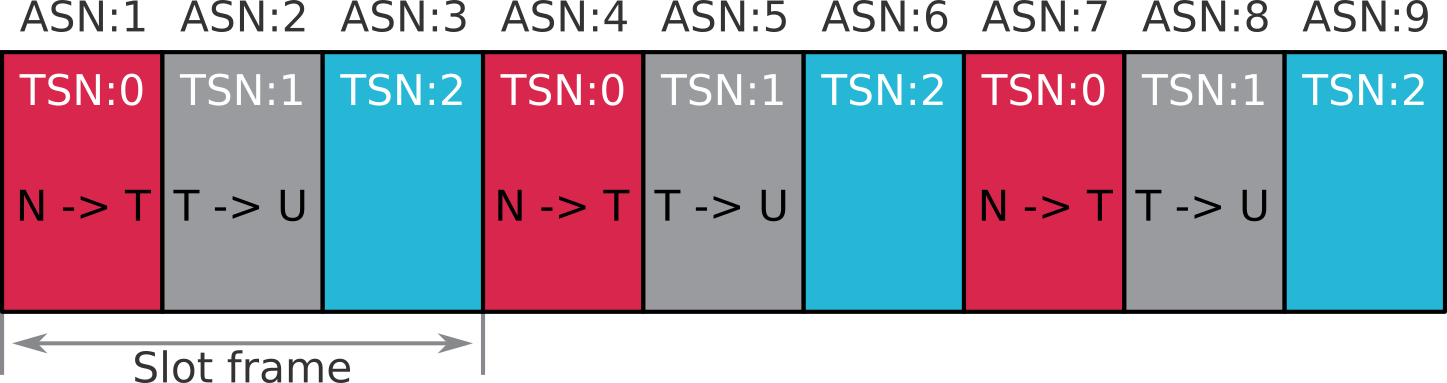
\includegraphics[scale=0.7]{res/pictures/sloframe.png}
  \caption{Slotframe.}
  \label{fig:state-slotframe}
\end{figure}

\subsubsection*{Channel Hopping}

TSCH peut utiliser 16 canaux différents numérotés de 0 à 15. Un lien entre deux noeuds dans TSCH est alors défini par la paire (timeslot, canal). Ainsi, chaque slot frame est divisiée par le nombre de canaux utilisé dans le réseau (Fig.~\ref{fig:state-tsch}). figure~\ref*{fig:state-slotframe}  Soit f la fréquence utilisée pour la communication entre deux noeuds:

\[
    f = F[(ASN + channel Offset)\% N_{channels}]
\]

où $N_{channels}$ est le nombre de canaux utilisés pour le réseau. F peut être vue comme une table qui contient une séquence de canaux.

\begin{figure}[H]
    \centering
    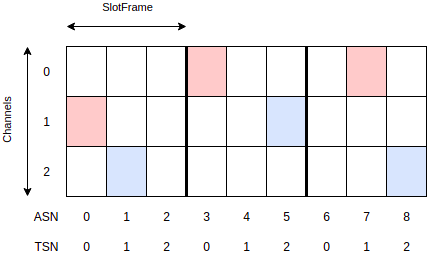
\includegraphics[scale=0.5]{res/pictures/tsch.drawio.png}
    \caption{Time Slotted Channel Hopping.}
    \label{fig:state-tsch}
\end{figure}


%\subsubsection*{Formation du PAN}

%\subsubsection*{Synchronisation en temps}
%%%%%%%%%%%%%%%%%%%%% glossaries %%%%%%%%%%%%%%%%%%%%%
%\printglossaries

%%%%%%%%%%%%%%%%%%%%% bibliography %%%%%%%%%%%%%%%%%%%%%
\bibliography{bibliography}{}
\bibliographystyle{plain}

%%%%%%%%%%%%%%%%%%%%% notes %%%%%%%%%%%%%%%%%%%%%
%<type>:<chapter_label_name>-<label>
%types:
% - chap: chapter
% - sec: section
% - subsec: sub section
% - fig: pictures
% - tb: tables
% - ft: foot notes
%
% chapters:
% - intro
% - state
%
%%%%%%%%%%%%%%%%%%%%% structure %%%%%%%%%%%%%%%%%%%%%
% TODO
%
\end{document}
